\section{Naive Bayes}
Naive Bayes algoritması, olasılık teorisine dayalı bir makine öğrenimi ve istatistiksel sınıflandırma algoritmasıdır. Temel olarak, bir nesnenin belirli bir sınıfa ait olma olasılığını tahmin etmek için kullanılır. Bu sınıflandırma algoritması, Bayes Teoremi'ne dayanır ve "naif" (ingenuous) olarak adlandırılır, çünkü sınıf tahminindeki özellikler arasındaki bağımsızlık varsayımı yapar, yani her özelliğin sınıfı etkileme olasılığı birbirinden bağımsızdır.

\begin{figure}[h]
    \centering
    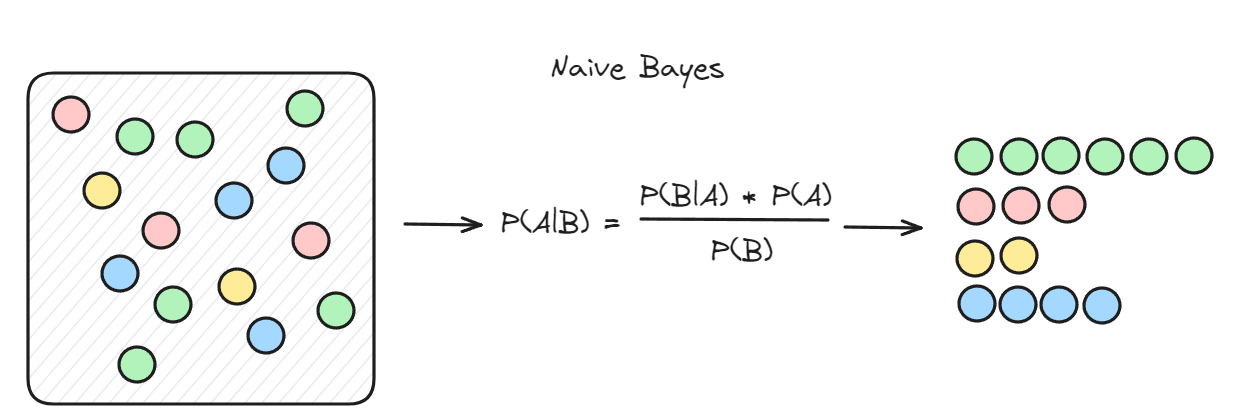
\includegraphics[width=1\textwidth]{images/naive_bayes.png}
    \caption{Naif bayes sınıflandırıcı.}
    \label{fig:enter-label}
\end{figure}

\subsection{Bayes Türleri}
\begin{itemize}
    \item \textbf{Gaussian Naive Bayes:} Özellikler sürekli değer (continuous value) ise bu değerlerin bir gauss dağılımı veya diğer bir değişle normal dağılımdan örneklendiğini varsayar.
    \item \textbf{Multinominal Naive Bayes:} Çok sınıflı kategorileri sınıflandırmak için kullanılır.
    \item \textbf{Bernoulli Naive Bayes:} Multinominal Naive Bayes’e benzer şekilde sınıflandırma yapar. Ancak tahminler sadece ikili şekildedir.
\end{itemize}

\newpage